\section{Schwingungsmoden}
Die Mode beschreibt eine bestimmte zeitliche stationäre Eigenschaft einer Welle (stehende Welle).
Die Form der Moden wird meist durch Randbedingungen bestimmt.\\
Bei elektro-magnetischen Wellen unterscheidet man folgende Moden-Formen \citep[vgl.][]{laser}:
\begin{itemize}
    \item \textbf{TEM}:
    Elektrische und magnetische Feldkomponente stehen senkrecht zur Ausbreitungsrichtung.
    \item \textbf{TE}:
    Elektrische Feldkomponente steht senkrecht zur Ausbreitungsrichtung. Die magnetische Feldkomponente zeigt in Ausbreitungsrichtung.
    \item \textbf{TM}:
    Magnetische Feldkomponente steht senkrecht zur Ausbreitungsrichtung. Die elektrische Feldkomponente zeigt in Ausbreitungsrichtung.
\end{itemize}
Bei den Lasermoden unterscheidet man grundsätzlich zwischen den axialen und transversalen Moden:
\subsection{Axialmoden}
Bei Axialmoden ist die Ausbreitungsrichtung entlang der optischen Achse des Resonators.
Im Resonator bilden sich nur stehende Wellen, d.h. es können nur bestimmte Frequenzen, deren Vielfaches der halben Wellenlänge der Resonatorlänge entspricht, anschwingen.
Das Spektrum kann aus diesem Grund nicht kontinuierlich sein, sondern diskret, die sogenannten Moden. \\
\textbf{Abstand Axialer Moden:}\\
Für den Abstand zweier Axialmoden nehmen wir die Bedingung für ein Verstärkung innerhalb des Resonators her:
\begin{equation}
    L=k\frac{\lambda}{2}
\end{equation}
Hier steht $L$ für die Länge des Resonators, $\lambda$ der Wellenlänge des emittierten Lichts und $k$ für eine natürliche Zahl.
Setzen wir nun für die Wellenlänge $c'=\nu\lambda$, mit $c'$ der Ausbreitungsgeschwindigkeit im Medium $c=c'n$ folgt:
\begin{align}
    L&=k\frac{\lambda}{2}\\
    L&=k\frac{c'}{2\nu}\\
    \nu&=\frac{ck}{2Ln}
\end{align}
Nun Bertrachen wir den Abstand zweier benachbarter Moden:
\begin{align}
    \nu_{k+1}-\nu_k&=\frac{c(k+1)}{2Ln}-\frac{ck}{2Ln}\\
    \Delta \nu =&\nu_{k+1}-\nu_k =\frac{c}{2Ln} \label{a}
\end{align}
Wie man erkennen kann, ist der Modenabstand, im Frequenzraum, bei allen gleich. 
Eine Mode ist nur dann in der Lage anzuschwingen wenn sie im Verstärkungsprofil des Laser liegt, dieses
ist begrenzt und somit können nicht unendlich viele Moden schwingen. \citep[vgl.][]{Laser-Dem}\\
Im nach folgendem Bild \ref{fig:Amode} ist das Verstärkungsprofil eingezeichnet \citep[vgl.][]{laser}:
\begin{figure}[h]
    \centering
    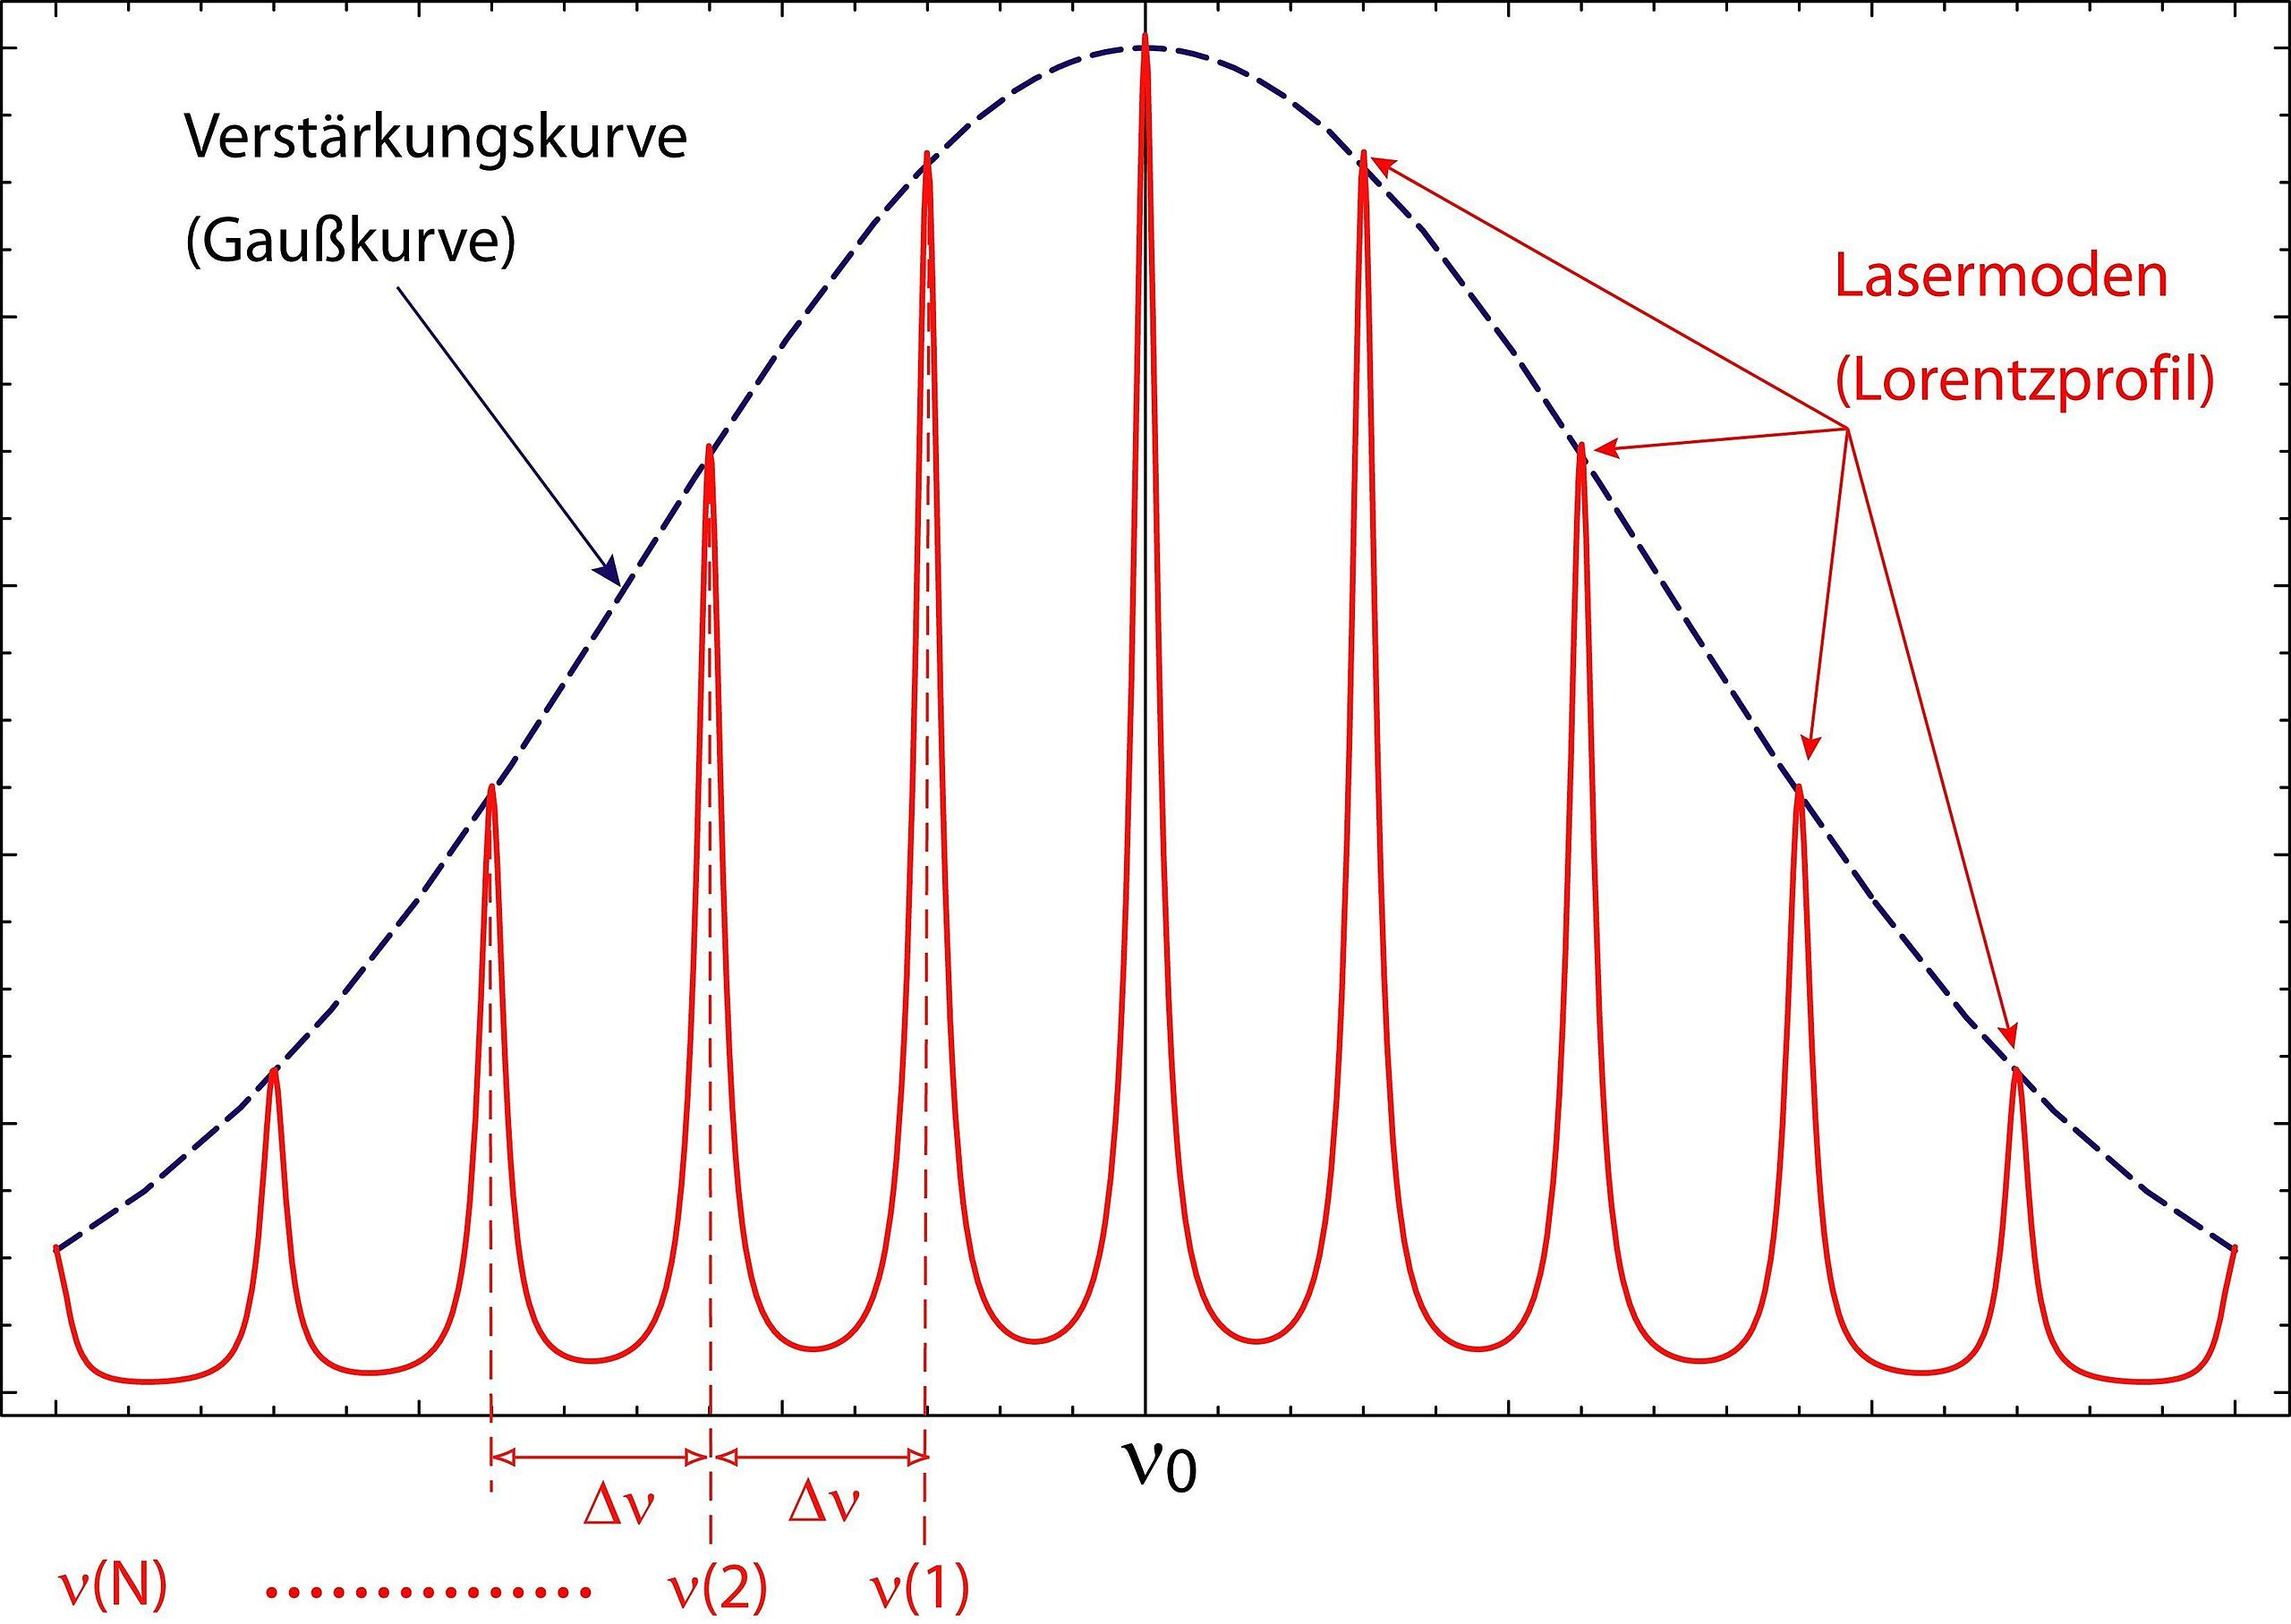
\includegraphics[width=0.55\textwidth]{FzV/LaserModes.jpg}
    \caption{Axiale Moden im Verstärkungsprofil}
    \label{fig:Amode}
\end{figure}\\
Die Bandbreite ist die Halbwertsbreite der Lasermoden im Frequenzraum. Ein Laser funktioniert nur dann, wenn die Bandbreite kleiner ist als die Verstärkung.


\subsection{Transversale Moden}
Diese Moden entstehen, wenn der Laserstrahl die Spiegel, beispielsweise im Resonator, nicht richtig trifft.
Zustande kommen die transversalen Moden durch falsche Justage der Spiegel, aber auch durch Verunreinigung der 
optischen Bauelemente. \\
Im Resonator kommt es zusätzlich zu einem oder mehreren unabhängigen Laserstrahlen, die in unterschiedlichen Winkeln auftreffen.
Es bilden sich stehende Wellen, die im Laserprofil Knoten aufweisen.\\
\newpage
Im Folgenden sind einige Beispiele für Transversale Moden:
\begin{figure}[h]
    \centering
    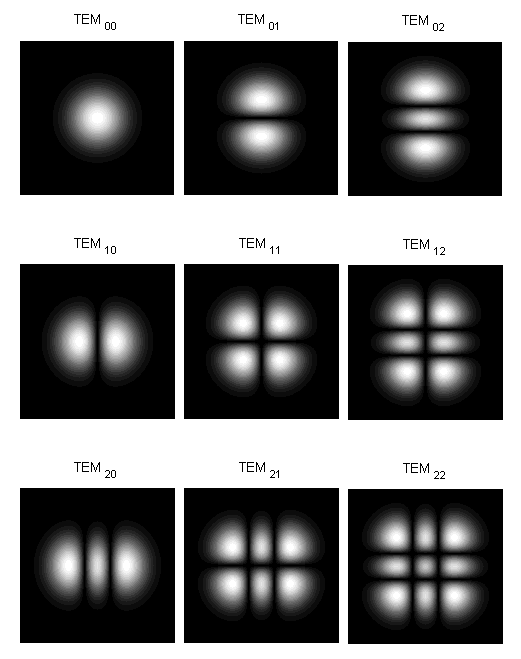
\includegraphics[scale=0.4]{FzV/TEM.png}
    \label{fig:Tmode}
    \caption{Verschiedene Transversale Moden}
\end{figure}\\
Gekennzeichnet sind die Lasermoden mit $TEM_{xy}$. Der Index x steht hierbei für die Anzahl ihrer Knotenlinien in x-Richtung
und der Index y für die Knotenlinien in y-Richtung. Die Grundmode $TEM_{00}$, zeigt im Idealfall ein Gauß-Profil. \citep[vgl.][]{laser}


\subsection{Single-Mode Laser}
Wenn man einen Laser mit einer hohen Wellenlängenstabilität benötigt, greift man oft auf einen single-mode Laser zurück.
Diese oszillieren nur auf einer Resonator-Eigenschwingung und geben somit nur eine Mode von sich.
Praktisch wird dies so umgesetzt, dass der Laserstrahl ein sogenanntes Fabry-Perot-Etalon\footnote{Dünnes, beidseitig verspiegeltes Blättchen. Funktionsweise ähnlich zum Fabry-Perot-Interferometer} trifft und dieses nur minimale Frequenzen durchlässt.
Da so nur eine Mode durchkommt hat man eine sehr hohe Wellenlängenstabilität. \citep[vgl.][]{Laser-Dem}
